\subsection{Processor}

The processor is modeled very similar to the design of the simple MIPS processor presented in Chapter 4.4 of the Curriculum Book (bibref). The largest change is that the instruction and data memory is not internal to the processor. The communication with memory is done through the ports of the processor. This relates to Figure 3.2 from the compendium (bibref). 

\begin{figure}[h]
	\centerline{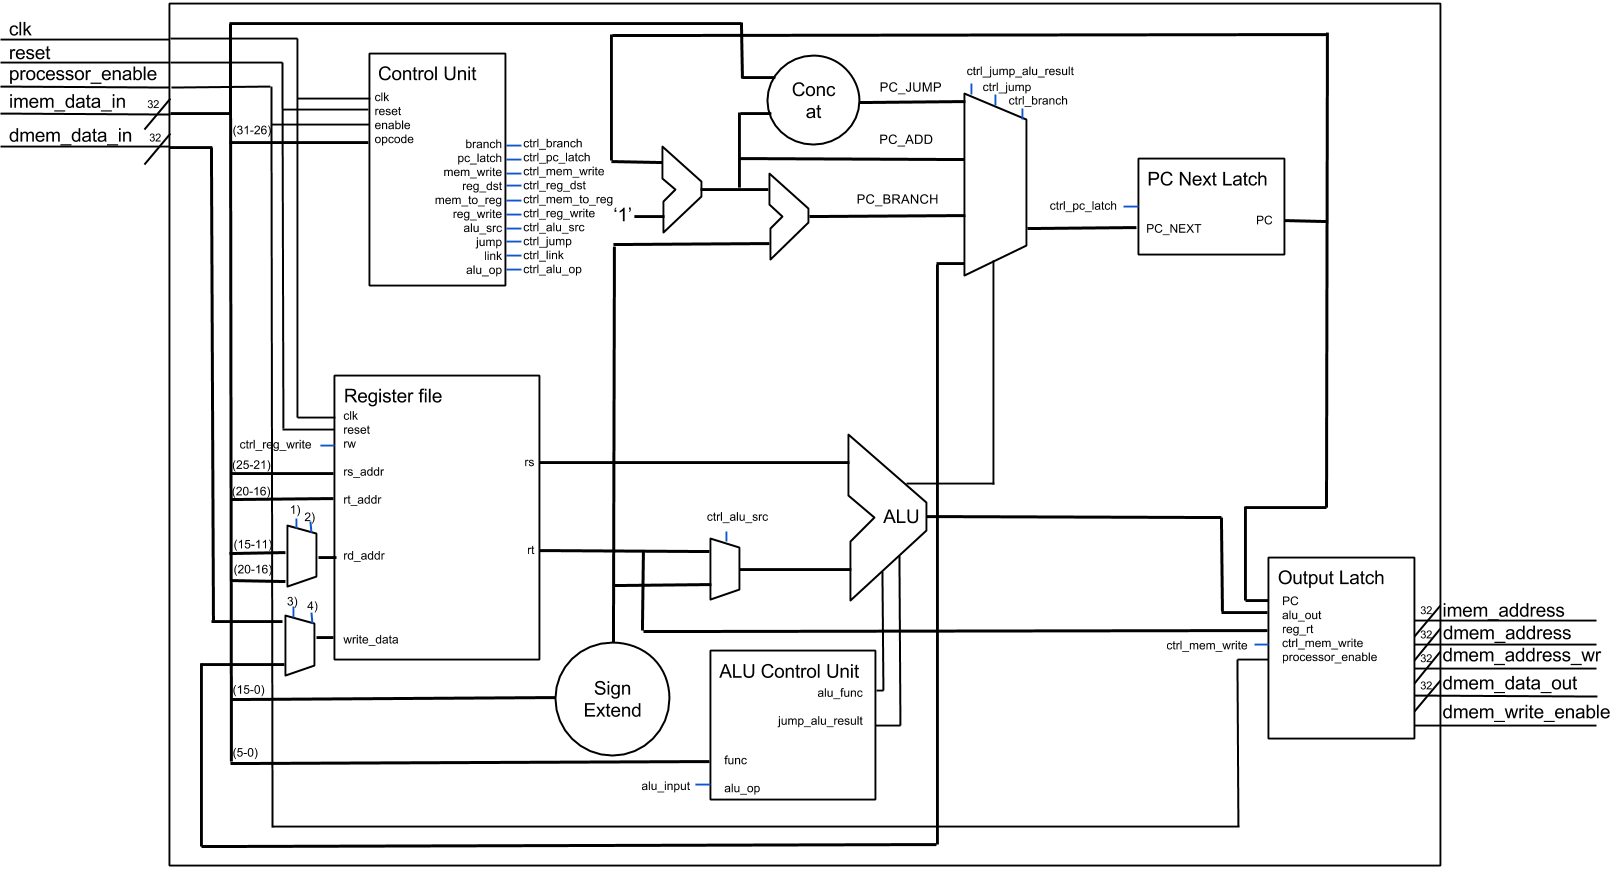
\includegraphics[width=550px]{figures/processor.png}}
	\caption{Processor}
\end{figure}

The implementation of the processor is located in the processor.vhd file. Here the core components of the processor, including the ALU, register file, control unit and alu control unit, are connected to each other. The components to take note of in this module is are the muxes and latches. The rest are simple wiring. 

\subsubsection{Program Counter}
The Program Counter is represented by the PC signal. It is connected to the imem\_address output bus and is incremented by 1 word each cycle. The usual MIPS PC is defined to be incremented by 4 bytes each cycle, but given the fact that the memory module in this assignment addresses words instead of bytes, the PC is incremented by 1. Logic exists in this module to perform jump and branch instructions. 

\paragraph{pc\_mux} This mux lets the processor implement the different types of jump and branch instructions. It sets the PC\_NEXT signal to either alu\_out, PC\_JUMP, PC\_BRANCH or PC\_ADD. 

\paragraph{next\_pc\_latch} This latch enables the control unit to make sure that the PC is not incremented before the processor reaches the state fetch in the start of each cycle. 

\subsubsection{Managing the register file}

This is where our extra feature jump and link comes in to play in the design. If the instruction is jal is executed the address PC+1\footnote{The MIPS specification states PC+8, but as the processor is not pipelined the branch delay slot was not implemented.} should be saved into r31.

\paragraph{req\_write\_mux} This mux multiplexes the different inputs for which register to write to. Possible values are x and y parts of the instruction and LINK\_REG used by the jal instruction. 

\paragraph{data\_write\_mux} This mux is responsible for choosing the correct input to write to the register selected by the previous described mux. It selects the dmem\_data\_in bus for store instructions and otherwise it's set to the output of the ALU. The exception is the extra feature when the PC\_ADD signal is stored in the LINK\_REG for the Jump And Link instruction.

\subsubsection{Driving the outputs}

\paragraph{drive\_output\_signals} This latch prevents the processor from driving its output signals when processor\_enable is not asserted. 
